\documentclass{beamer}
\pdfstringdefDisableCommands{%
  \def\\{}%
  \def\texttt#1{<#1>}%
}
\beamertemplatenavigationsymbolsempty


% Footnote
\setbeamertemplate{footline}{\leavevmode%
  \begin{beamercolorbox}[wd=.33\paperwidth,left,ht=2.5ex,dp=1.5ex,rightskip=4pt plus 1pt, leftskip=4pt]{subsection in head/foot}
    Team 12
  \end{beamercolorbox}%
  \begin{beamercolorbox}[wd=.33\paperwidth,center,ht=2.5ex,dp=1.5ex]{section in head/foot}
  \end{beamercolorbox}%
  \begin{beamercolorbox}[wd=.34\paperwidth,ht=2.5ex,dp=1.5ex,leftskip=4pt plus 1pt,rightskip=4pt plus 1pt]{subsection in head/foot}
    \hfill\insertframenumber/\inserttotalframenumber
  \end{beamercolorbox}%
}


\title{Stato di avanzamento}
\subtitle{Sprint 2}
\author{
  \texorpdfstring{\parbox{45mm}{\centering\scriptsize Zaid Cheikh Ibrahim \\[-0.3em] {\tiny PO Operativo}}}{} \and 
  \texorpdfstring{\parbox{45mm}{\centering\scriptsize Tian Cheng Xia \\[-0.3em] {\tiny Scrum master}}}{}\\[1em]
  \texorpdfstring{\parbox{45mm}{\centering\scriptsize Qun Hao Henry Lee \\[-0.3em] {\tiny Developer}}}{} \and 
  \texorpdfstring{\parbox{45mm}{\centering\scriptsize Manuel Paris \\[-0.3em] {\tiny Developer}}}{}\\
}
\institute{
  Corso di Ingegneria del Software\\
  Alma Mater Studiorum $\cdot$ Università di Bologna  
}
\date{15 novembre 2022}


\begin{document}

{
\setbeamertemplate{footline}{} 
\begin{frame}
  \titlepage
\end{frame}
}
\addtocounter{framenumber}{-1}

\begin{frame}
  \frametitle{Obiettivi dello sprint}
  \begin{itemize}
    \item Implementare le richieste emerse allo sprint review precedente
    \item Concludere l'epica riguardante la visualizzazione e l'analisi dei tweet
  \end{itemize}
\end{frame}

\begin{frame}
  \frametitle{Use case}
  \begin{figure}
    \centering
    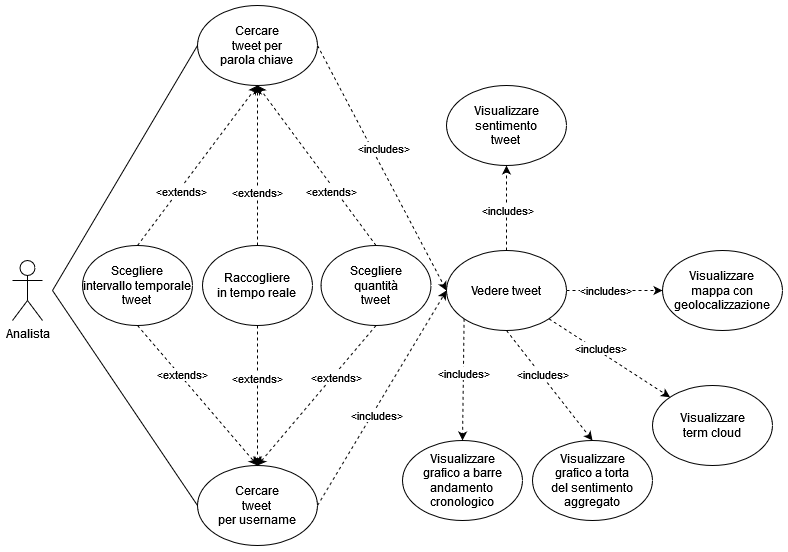
\includegraphics[width=\textwidth]{./img/usecase.png}
  \end{figure}
\end{frame}

\begin{frame}
  \frametitle{Pre-retrospettiva}
  \begin{figure}
    \centering
    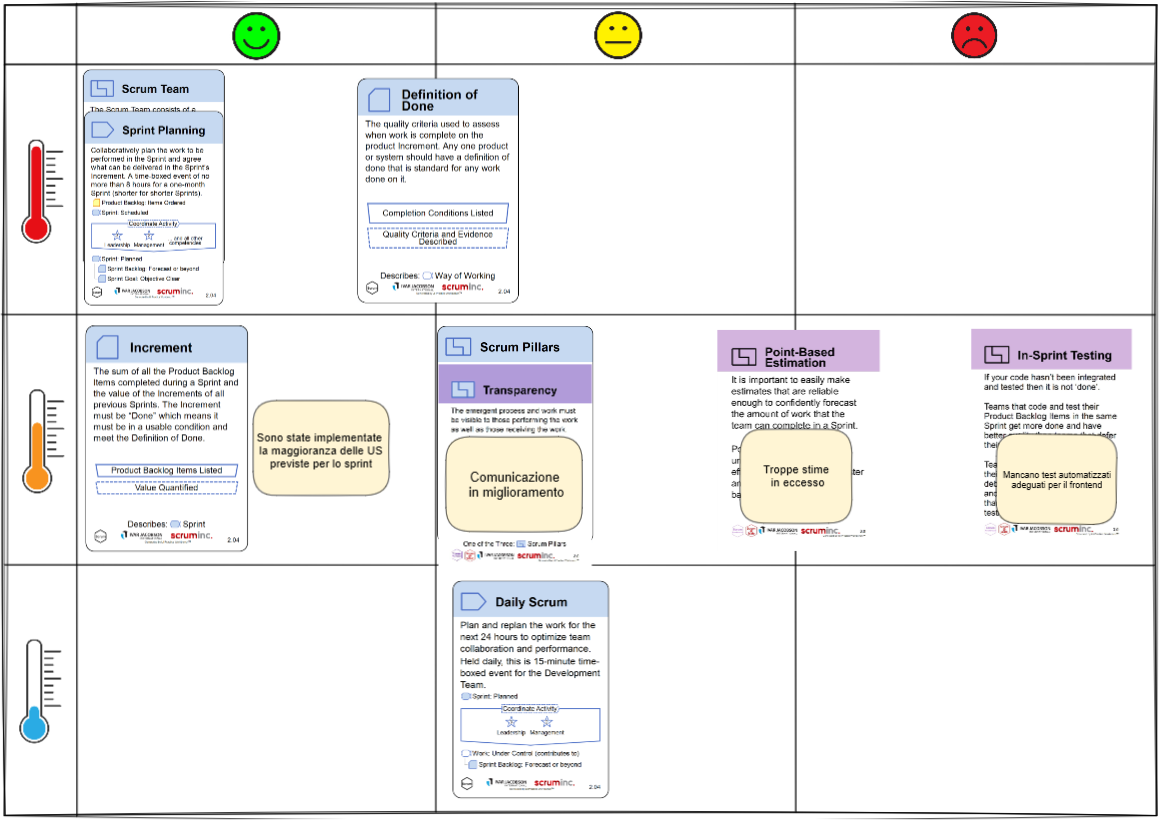
\includegraphics[width=\textwidth]{./img/preretrospettiva.png}
  \end{figure}
\end{frame}

\begin{frame}
  \frametitle{Stato attuale}
  \begin{itemize}
    \item Possibilità di selezionare il numero di tweet da raccogliere con una singola richiesta
    \item Ricerca dei tweet per intervallo temporale
    \item Ricerca dei tweet per parola chiave
    \item Visualizzazione su mappa dei dati di geolocalizzazione dei tweet
    \item Possibilità di raccogliere tweet in tempo reale
  \end{itemize}
  \begin{figure}
    \centering
    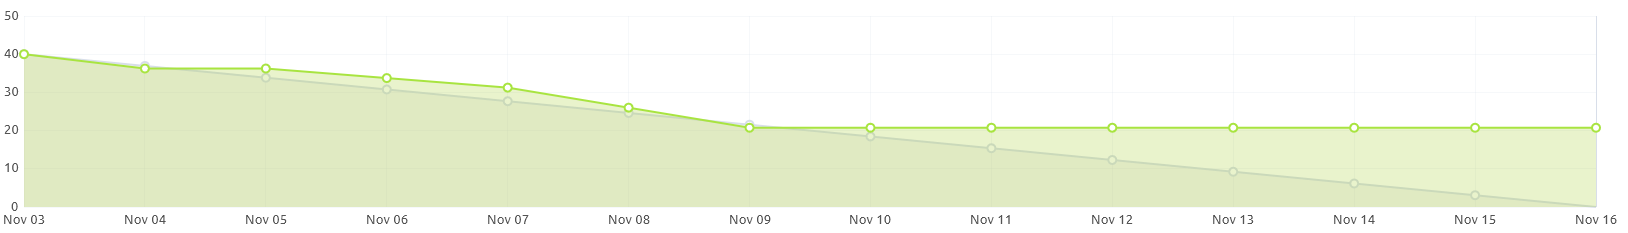
\includegraphics[width=\textwidth]{./img/burndown.png}
    \caption{Burndown sprint 2}
  \end{figure}
\end{frame}

\end{document}